\documentclass[varwidth=40cm]{standalone}
\usepackage{tikz}
\usepackage{style}

\def\from{0}
\def\to{4.5}

\begin{document}
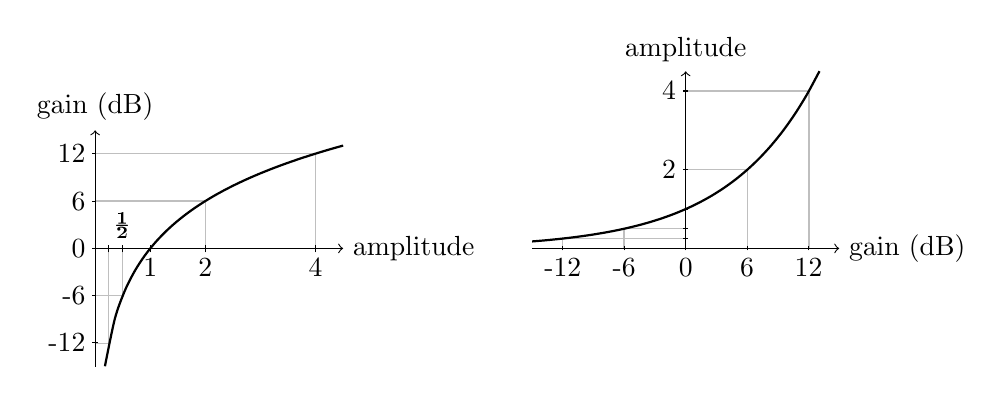
\begin{tikzpicture}
  \begin{scope}[xscale=.7,yscale=.1]
    \foreach \y in {-12,-6,0,6,12} {
      \draw (\from,\y) node [left] {\y};
      \draw (\from-.05,\y) -- (\from+.05,\y);
    }
    \foreach \x in {.25,.5,1,2,4} {
      \draw [lightgray] (\x,0) -- (\x,{20*log10(\x)}) -- (\from,{20*log10(\x)});
      \draw (\x,-.5) -- (\x,.5);
    }
    \foreach \x in {1,2,4} {
      \draw (\x,0) node[below] {\x};
    }
    \draw (.5,0) node[above] {\textonehalf};
    % \draw (.25,0) node[above] {\textonequarter};
    \draw[thick, smooth, domain=.178:\to] plot ({\x}, {20*log10(\x)});
    \draw[->] (\from,0) -- (\to,0) node[right] {amplitude};
    \draw[->] (\from,-15) -- (\from,15) node[above] {gain (dB)};
  \end{scope}

  \begin{scope}[shift={(7.5,0)},xscale=.13,yscale=.5]
    \foreach \y in {.25,.5,1,2,4} {
      \draw[lightgray] (0,\y) -- ({20*log10(\y)},\y) -- ({20*log10(\y)},0);
      \draw (-.25,\y) -- (.25,\y);
    }
    % \draw (0,1) node [left] {1};
    \draw (0,2) node [left] {2};
    \draw (0,4) node [left] {4};
    \foreach \x in {-12,-6,0,6,12} {
      \draw (\x,-.05) -- (\x,.05);
      \draw (\x,0) node[below] {\x};
    }
    \draw[thick, smooth, domain=-15:13.07] plot ({\x}, {pow(10,\x/20)});
    \draw[->] (-15,0) -- (15,0) node[right] {gain (dB)};
    \draw[->] (0,0) -- (0,4.5) node[above] {amplitude};
  \end{scope}
\end{tikzpicture}
\end{document}
